\chapter{Introduction}
\label{chap:introduction}
This is a citation: \cite{patchCore2022}


This is a figure: 

\begin{figure}[ht]
    \centering
    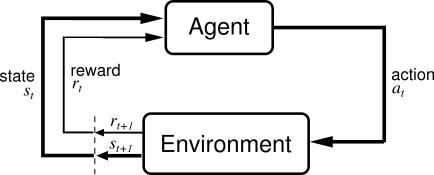
\includegraphics[width=.5\textwidth]{figures/AgentEnviornment.png}
    \caption{I am a caption}
    \label{fig:my_label}
\end{figure}



- It is important to note somewhere in the paper that we are dealing with very high variance in our ensemble since we only have 5 models ish

Concept for introduction:
- General approach -> Start very wide and narrow it down

- we are in manuacturing setting -> quality control of metal parts
-> write one sentence about industrial revolution and address the rising needs for metal parts lately(find credible numbers of metal parts production) 
- say that most things we engineer nowadays has strict requirements and needs to be functioning properly to avoid dangerous situations/fatalities etc
- one of many problems of this requirement is that parts may be insufficiently produced which can lead to unecpected breakage/ausfällen

- to combat this, people have startet inspecting produced parts with different approaches. Yet all approaches required extensive human labor
- in recent decades with the rise of computers alongside computer vision advancements, this quality controll process has often been automated 
  whereever possible
- Mention that the striving for increasingly accurate controls brought forth the field of anomaly detection which has been a very popular 
  and ectensively researched topic in the last couple of years
- The subfield of specifically image anomaly detection aims at successfullly distinguishing between images of good /normal and 
  anomalous parts.
- nochmal bezug auf manufacturing

- erklären dass es verschiedene arten von IAD gibt -> bspw. image detection and anomaly localization
- auch logical vs structural anomalies anreißen

- sagen dass IAD best performance eig unsupervised sind weil Gründe(= große data imbalance, wenig data overall, etc...(maybe noch einer aber 3 gründe reichen))
- irgendwo erwähnen dass IAD aktuell sehr gute ergebnisse erzielt

- Eventuell kurz auch arten von IAD (embedding vs reconstruction) anschneiden? aber nicht zu detailiert weil der rest kommt in background

- gegen ende aber probleme aufzählen 
-> gute ergebnisse sind meist in sehr klinischen settings nur beobachtbar
-> localization bislang schwieriger als image detection
-> ansätze welche gut sind performen doch deutlich schlehter bei logical anomalies, ergebnisse oft inkonsistent
-> logical anomalies sind aber wichtig weil sie neue felder der quality control ermöglichen

- Damit einleiten in die contributions





\section{Begin Intro}
In recent years, image anomaly detection has become significantly more important among many scientific communities, especially in industrial applications. This is no surprise, considering the
amount of mechanically manufactured parts in factories all over the world. Since in most parts of the world, manufactured items undergo rather strict regulations and are expected to work
in real case scenarios, there is a need for sufficient quality control, that is rising with the amount of produced components. A long time ago, it has come to a point where human based quality 
checks are not adequate anymore for the production volume, which has led to computer solutions for the problem. Generally speaking, anomaly detection has first been proposed in 1986 for 
intrusion detection systems(referenz). While the methods and modalities may change, the high level idea stays the same: Detecting data that deviates from a set standard to a degree that is becoming
problematatic regarding the own requirements(letzer part maybe neu formulieren). Besides many approaches that were used over the years, deep learning approaches for image anomaly detection have
become very popular lately. A likely reason for this are impressively high performance scores with state of the art models achieving an area under the receiver operateor curve of around 0.96 and 
sometimes even more.
It is difficult to say what the first deep learning approaches to this topic were(fact checking), but a notable milestone is definetly Bergmann 2021(Referenz). Among blabla, they introduced
the MVTecAD dataset which is used widely and serves as a dataset to benchmark on for nearly every IAD paper released afterwards. - Übergang benötigt

\section{Table Test Viz}

This is a table:
\begin{table}[htbp]
    \tiny
    \centering
    \begin{tabularx}{\textwidth}{|X|X|X|}%{|c|p{5cm}|p{5cm}|p{5cm}|}
        \hline
        \textbf{Metric/Level} & \textbf{Formula} & \textbf{Remarks/Usage} \\
        \hline
        Precision (P) $\uparrow$ & $P = TP/(TP + FP)$ & True Positive (TP), False Positive (FP) \\
        \hline
        Recall (R) $\uparrow$ & $R = TP/(TP + FN)$ & False Negative (FN), True Positive Rate (TPR) \\
        \hline
        True Positive Rate (TPR) $\uparrow$ & $TPR = TP/(TP + TN)$ & True Negative (TN) \\
        \hline
        False Positive Rate (FPR) $\downarrow$ & $FPR = FP/(FP + TN)$ & True Negative (TN) \\
        \hline
        Area Under the Receiver Operating Characteristic curve (AU-ROC) $\uparrow$ & $ \int_{0}^{1} (TPR) \: d(FPR)$ & Classification \\
        \hline
        Area Under Precision-Recall (AU-PR) $\uparrow$ & $\int_{0}^{1} P \: d(R)$ & Localization, Segmentation \\
        \hline
        Per-Region Overlap (PRO) $\uparrow$ & $PRO = \frac{1}{N} \sum_{i} \sum_{k} \frac{P_i \cap C_{i,k}}{C_{i,k}}$ & Total ground-truth number (\(N\)), Predicted abnormal pixels (\(P\)), Defect ground-truth regions (\(C\)) \\
        \hline
        Saturated Per-Region Overlap (sPRO) $\uparrow$ & $sPRO(P) = \frac{1}{m} \sum_{i=1}^{m} \min(\frac{A_i \cap P}{s_i}, 1)$ & Total ground-truth number (\(m\)), Predicted abnormal pixels (\(P\)), Defect ground-truth regions (\(A\)), Corresponding saturation thresholds (\(s\)) \\
        \hline
        F1 Score $\uparrow$ & $F1 = 2(P \cdot R)/(P + R)$ & Classification \\
        \hline
        Intersection over Union (IoU) $\uparrow$ & $IoU = (H \cap G)/(H \cup G)$ & Prediction (H), Ground truth (G)/ Localization, Segmentation \\
        \hline
    \end{tabularx}
    \caption{Description of metrics}
    \label{tab:metrics}
\end{table}






\section{Contributions}
This research provides multiple contributions to the field of image anomaly detection, in an effort to further push the progress of 
robust anomaly localization in differnt domains. 

1. To address the problems mentioned at the end of the last section, we attempt (vllt ohne attempt wenn der ansatz funzt) 
to build a heterogeneous feature level ensemble network, combining differnt state of the art IAD approaches, with the goal to improve 
general performance but also robustness in image localization. This ensemble network is tested on its performance regarding structural 
but also logical anomalies from differnt parts. 
2. Furtheremore an extensive study on the performance of a wide ranging selection of IDA methods on the MVTecAD LOCO dataset is performed. 
This serves to highlight the current state of anomaly detection in logical problems, and also investigate the application potential of 
those approaches in such domains(den satz mag ich nicht). (vllt noch einbauen dass diese experimente ggf noch nie durchgeführt wurden und auch code bereitgestellt wird)
3. Lastly we introduce a new category to the MVTecAD LOCO dataset to further increase the diversity of this dataset and strengthen the focus 
of this thesis on metal maufactured parts.
4. The mentioned network and experiments are also streamlined(checken ob ich das wort richtig benutzt hab) into an easy to use pipeline 
to be used for future experiments in that area.

The contributions mentioned firstly benefit faster research entry and an accelerated experimentation process, with an intuitive setup, 
as well as potential industrial applications. 
Furthermore they give more insight into the capabilities of existing methods in an industrial setting and thus also provide a more 
various and practical setting than the prior categories in the MVTecAD(referenz) dataset. The same methods are also testet on their limitations 
regarding logical anomalies which was earlier made out to be a relevant aspect of anomaly detection in current manufacturing quality control 
settings. Lastly through the use of a robust ensemble approach for heterogeneous classifers, this opens up possibilities for expanding 
the field of application of SOTA IAD methods to other domains with robust performance and may also produce more usable results in real 
world IAD settings. The presented network can also be used as ground work(fundament oder synonym oder so) for future experiments in 
different directions. For example, the pipeline may be efficiently used to start investigations on multiperspective datasets in anomaly 
detection, a topic that also could further advance current IAD applciations.




-- in my work i contribute the following things:
- pipeline to infer new images on different algorithms and compare them
-> pipeline is industry focussed for benefits of the guys where i write my thesis

- research on multi perspective detection

- research of ensemble output learning to enhance individual network performance
-> simple network over 5-6 outputs

- introduction of very new dataset categories in style of mvtec LOCO dataset

